%\documentclass[trans]{beamer}
\documentclass[9pt]{beamer}

% Try the class options [notes], [notes=only], [trans], [handout],
% [red], [compress], [draft], [class=article] and see what happens!

% Copyright 2003 by Till Tantau <tantau@users.sourceforge.net>.
%
% This program can be redistributed and/or modified under the terms
% of the LaTeX Project Public License Distributed from CTAN
% archives in directory macros/latex/base/lppl.txt.

% For a green structure color use:
%\colorlet{structure}{green!50!black}

%%%%%%%%%% User macros%%%%%%%%%%%
\newcommand{\mypurple}[1]{{\color[rgb]{0.7,0,0.8}#1}}
\newcommand{\myred}  [1] {{\color{red}#1}}
\newcommand{\myblue} [1] {{\color{blue}#1}}
\newcommand{\mygreen}[1] {{\color[rgb]{0,0.5,0}#1}}
\newcommand{\Nat}{\mathbb{N}}
\def\sla  {\!\!\!\slash}
%%%%%%%%%%%%%%%%%%%%%%%%%%%%%%%%%
\mode<article> % only for the article version
{
  \usepackage{beamerbasearticle}
  \usepackage{fullpage}
  \usepackage{hyperref}
}

%\beamertemplateshadingbackground{red!10}{blue!10}
%\beamertemplateshadingbackground{blue!10}{blue!10}

%\usepackage{beamerthemeshadow}

\usepackage{pgf,pgfarrows,pgfnodes,pgfautomata,pgfheaps,pgfshade}
\usepackage{amsmath,amssymb}
\usepackage[latin1]{inputenc}
\usepackage{colortbl}
\usepackage[english]{babel}
%\usepackage{verbatim}
%\usepackage{listings}
\usepackage[procnames]{listings}

%\usepackage{lmodern}
\usepackage[T1]{fontenc} 

\usepackage{times}

% for code colouring
\include{pythonlisting}
\include{cpplisting}
\usepackage{minted}

% Use some nice templates
\beamertemplatetransparentcovereddynamic
\usetheme{Binet}
%\usetheme{Madrid}
%\usetheme{Boadilla}
%\usetheme{Berkeley}
%\usetheme{Rochester}

%\def\command#1{\list{}{\leftmargin=2em\itemindent-\leftmargin\def\makelabel##1{\hss##1}}%
%\item\extractcommand#1@\par\topsep=0pt}
%\def\endcommand{\endlist}
%\def\extractcommand#1#2@{\strut\declare{\texttt{\string#1}}#2}

%
% The following info should normally be given in you main file:
%

\hypersetup{%
  pdftitle={go-fads},%
  pdfauthor={Sebastien Binet}
  %pdfsubject={AthenaMP},
  %pdfkeywords={ATLAS,Athena,python,COW,parallelization},
%  pdfpagemode=FullScreen%
}

\title[go-fads]{\texttt{fads}\\a (\texttt{Go}-based) FAst Detector Simulation toolkit}
\author[S. Binet]{S\'ebastien~Binet}%\inst{1}
\institute[LAL]{
%  \inst{1}%
  LAL/IN2P3}
\date{2015-01-21}

% \begin{center}
% On behalf of Core people
% \end{center}

\pgfdeclaremask{lal}{lal}
%\pgfdeclaremask{ubp}{UBP-logo}
\pgfdeclareimage[mask=lal,width=2cm]{lal-logo}{lal}
%\pgfdeclareimage[mask=ubp,width=1cm]{ubp-logo}{UBP-logo}

\logo{%
  \vbox{%
    \hbox{\pgfuseimage{lal-logo}}%
  }%
}


\begin{document}
\lstset{language=C++}

\frame{\titlepage
%  \hskip0.44\paperwidth
%  \insertlogo

    \begin{beamercolorbox}[sep=8pt,center]{mylogo}
      \usebeamercolor[fg]{mylogo}\insertlogo
    \end{beamercolorbox}

}

%\section*{Outline}
%\frame{\tableofcontents[part=1]}%,pausesections]}

%\AtBeginSubsection[]
%{
%  \frame<handout:0>
%  {
%    \frametitle{Outline}
%    \tableofcontents[current,currentsubsection]
%  }
%}

\part<presentation>{Main Talk}

%%%%%%%%%%%%%%%%%%%%%%%%%%%%%%%%%%%%%%%%%%%%%%%%%%%%%%%%%%%%%%%%%%%%%%%%%%%%%%%
%%%%%%%%%%%%%%%%%%%%%%%%%%%%%%%%%%%%%%%%%%%%%%%%%%%%%%%%%%%%%%%%%%%%%%%%%%%%%%%
%\section[Outline]{Outline}

% \frame<beamer>{
%   \frametitle{Outline}
%   \begin{columns}
% \begin{column}{0.49\textwidth}
%   \begin{block}{}
%   \tableofcontents
%   \end{block}
% \end{column}
% \end{columns}

% }
%\frame{\partpage}

%%%%%%%%%%%%%%%%%%%%%%%%%%%%%%%%%%%%%%%%%%%%%%%%%%%%%%%%%%%%%%%%%%%%%%%%%%%%%%%
%%%%%%%%%%%%%%%%%%%%%%%%%%%%%%%%%%%%%%%%%%%%%%%%%%%%%%%%%%%%%%%%%%%%%%%%%%%%%%%
\section[mysection]{mysection}

\frame{
  \frametitle{\texttt{fads}}

  \texttt{fads} is a \texttt{``FAst Detector Simulation''} toolkit.

  \begin{block}{}
    \begin{itemize}
    \item morally a translation of
      \myblue{\href{https://cp3.irmp.ucl.ac.be/projects/delphes}{\texttt{C++-Delphes}}}
      into \myblue{\href{https://golang.org}{\texttt{Go}}}

    \item a testbed for \texttt{R\&D} in
      \myblue{\href{https://golang.org}{\texttt{Go}}} and concurrent
      frameworks

      \item uses
        \myblue{\href{https://github.com/go-hep/fwk}{\texttt{go-hep/fwk}}}
        to expose, manage and harness concurrency into the usual
        \texttt{HEP} event loop (\texttt{initialize | process-events |
          finalize})
    \end{itemize}
  \end{block}

  \begin{block}{}
    Code is on \texttt{github} (\texttt{BSD-3}):
    \begin{itemize}
      \item \myblue{\href{https://github.com/go-hep/fwk}{\texttt{https://github.com/go-hep/fwk}}}
      \item \myblue{\href{https://github.com/go-hep/fads}{\texttt{https://github.com/go-hep/fads}}}
    \end{itemize}
  \end{block}

  \begin{block}{}
    Documentation is served by \myblue{\href{https://godoc.org}{\texttt{godoc.org}}}, Continuous Integration by \myblue{\href{https://drone.io/github.com/go-hep/fads/latest}{\texttt{drone.io}}}
        
    \begin{itemize}
    \item \myblue{\href{https://godoc.org/github.com/go-hep/fwk}{\texttt{https://godoc.org/github.com/go-hep/fwk}}}
    \item \myblue{\href{https://godoc.org/github.com/go-hep/fads}{\texttt{https://godoc.org/github.com/go-hep/fads}}}
    \end{itemize}
  \end{block}
}

\begin{frame}[fragile]
  \frametitle{\texttt{go-hep/fads} - Installation}

  \begin{block}{}
    As easy as:
\begin{minted}[]{sh}
$ export GOPATH=$HOME/dev/gocode
$ export PATH=$GOPATH/bin:$PATH

$ go get github.com/go-hep/fads/...
\end{minted}

    
  Yes, with the ellipsis at the end, to also install sub-packages.
  \end{block}

  \begin{block}{}
    \begin{itemize}
      \item \texttt{go get} will recursively download and install all
        the packages that
        \myblue{\href{https://github.com/go-hep/fads}{\texttt{go-hep/fads}}}
        depends on. (no \texttt{Makefile} needed)

      \item you get a \myred{statically linked} executable in a matter
        of seconds (even for large projects)
      \item \myred{simple} deployment and distribution
      \item the \mypurple{speed} of development of \texttt{python}
        with the \mypurple{speed} of execution of \texttt{C++}
    \end{itemize}
  \end{block}
\end{frame}

\frame{
  \frametitle{\texttt{go-hep/fwk} - Concurrency}
  \begin{block}{}
    \myblue{\href{https://github.com/go-hep/fwk}{\texttt{go-hep/fwk}}}
    enables:
    \begin{itemize}
    \item event-level concurrency
      \item tasks-level concurrency
    \end{itemize}
  \end{block}

\quad\\
 \myblue{\href{https://github.com/go-hep/fwk}{\texttt{go-hep/fwk}}}
  relies on \myblue{\href{https://golang.org}{\texttt{Go}}}'s runtime
  to properly schedule \mypurple{goroutines}.

\quad\\
 For sub-task concurrency, users are by construction required
    to use \myblue{\href{https://golang.org}{\texttt{Go}}}'s
    constructs (\texttt{goroutines} and \texttt{channels}) so
    everything is consistent \myred{and} the \mypurple{runtime} has
    the \myred{complete picture}.

    \begin{exampleblock}{}
      \emph{Note:} \myblue{\href{https://golang.org}{\texttt{Go}}}'s
      runtime isn't yet \texttt{NUMA}-aware.\\
      A proposal for \texttt{Go-1.5} (June-2015) is in the \myblue{\href{https://docs.google.com/document/d/1d3iI2QWURgDIsSR6G2275vMeQ_X7w-qxM2Vp7iGwwuM/pub}{\texttt{works}}}
    \end{exampleblock}
}

\begin{frame}[fragile]
  \frametitle{\texttt{go-hep/fads} - real world use case}

  \begin{block}{}
    \begin{itemize}
      \item translated
        \myblue{\href{https://cp3.irmp.ucl.ac.be/projects/delphes}{\texttt{C++-Delphes}}}'
        \textsc{Atlas} data-card into \texttt{Go}
      \item
        \myblue{\href{https://github.com/go-hep/fads/blob/master/cmd/fads-app/main.go}{\texttt{go-hep/fads-app}}}
      \item installation:
        \begin{minted}[]{sh}
$ go get github.com/go-hep/fads/cmd/fads-app
$ fads-app -help
Usage: fads-app [options] <hepmc-input-file>

ex:
 $ fads-app -l=INFO -evtmax=-1 ./testdata/hepmc.data

options:
  -cpu-prof=false: enable CPU profiling
  -evtmax=-1: number of events to process
  -l="INFO": log level (DEBUG|INFO|WARN|ERROR)
  -nprocs=0: number of concurrent events to process
        \end{minted}
    \end{itemize}
  \end{block}
\end{frame}

\frame{
  \frametitle{\texttt{go-hep/fads} - components}

  \begin{block}{}
    \begin{itemize}
      \item a \texttt{HepMC} converter
      \item  particle propagator
      \item  calorimeter simulator
      \item  energy rescaler, momentum smearer
      \item  isolation
      \item  b-tagging, tau-tagging
      \item  jet-finder (reimplementation of FastJet in Go: \myblue{\href{https://github.com/go-hep/fastjet}{\texttt{go-hep/fastjet}}})
      \item  histogram service (from \myblue{\href{https://github.com/go-hep/fwk}{\texttt{go-hep/fwk}}})

    \end{itemize}
  \end{block}

  \begin{exampleblock}{}
    Caveats:
    \begin{itemize}
      \item no real persistency to speak of (\emph{ie:} \texttt{JSON},
        \texttt{ASCII} and \texttt{Gob})

        \item jet clustering limited to $N^3$ (slowest and dumbest
          scheme of \texttt{C++-FastJet})
    \end{itemize}
  \end{exampleblock}
}

\frame{
\begin{center}
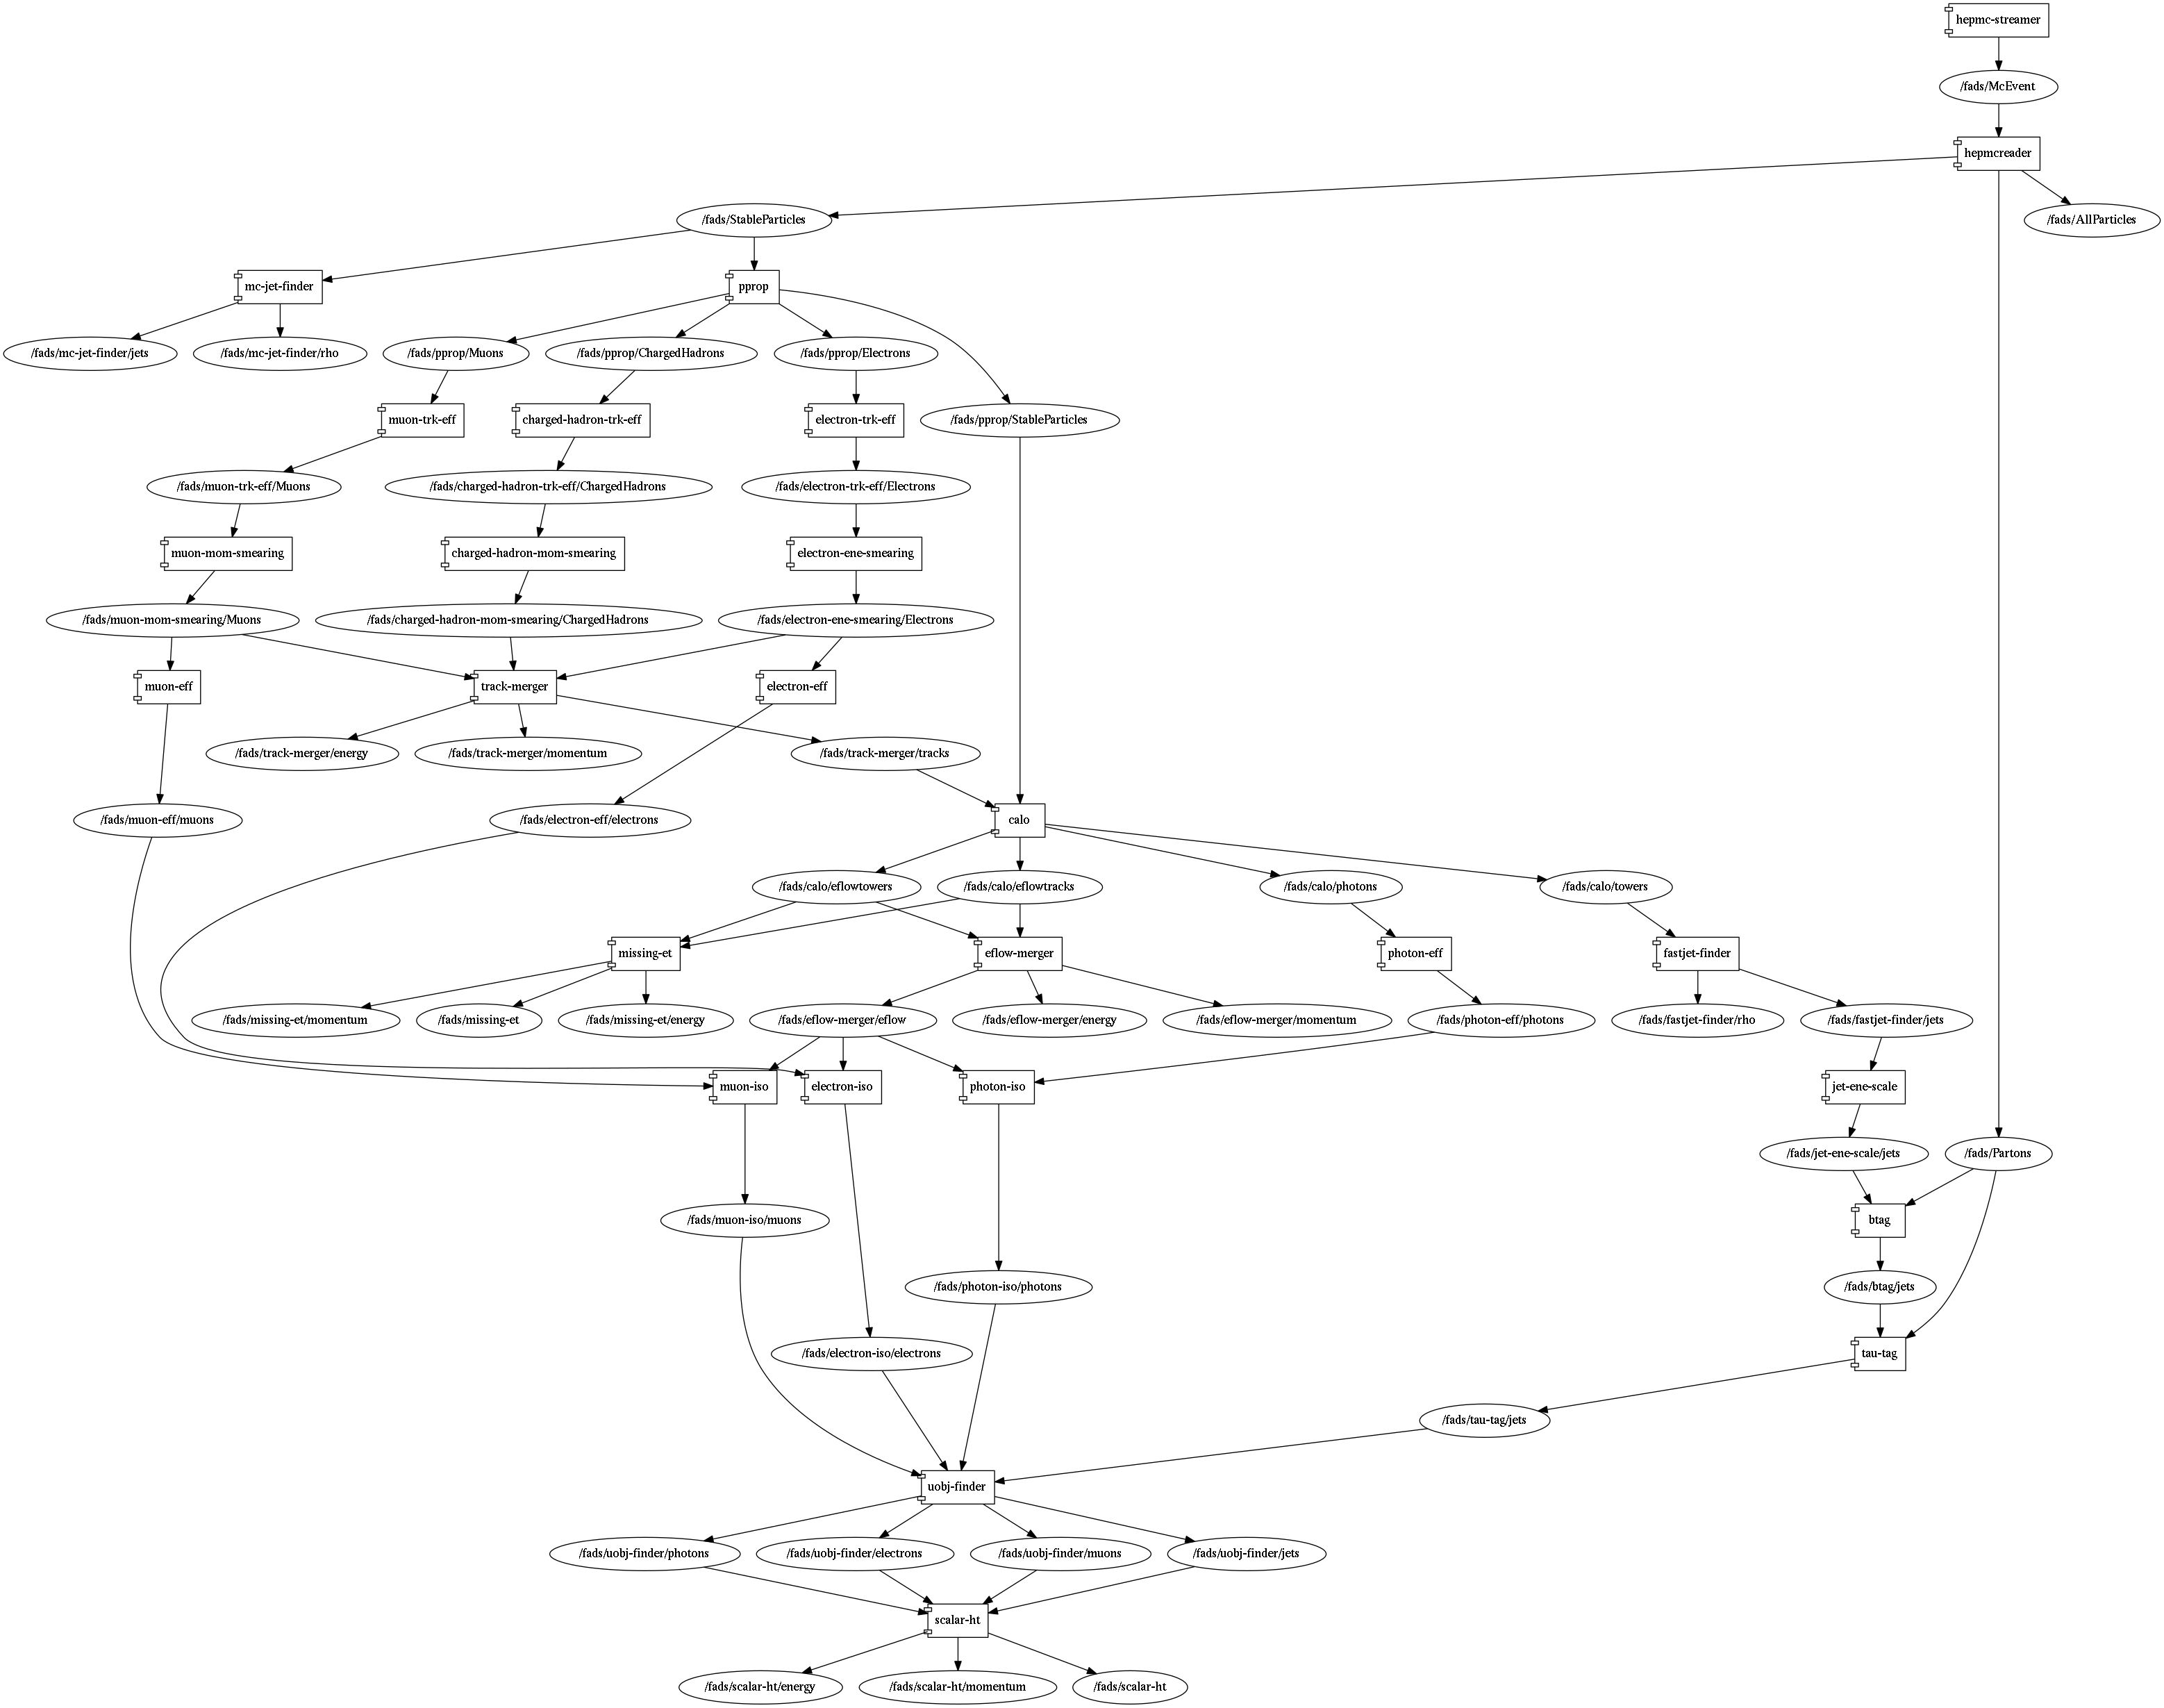
\includegraphics[width=0.95\linewidth]{figs/fads-dflow.png}
\end{center}
}

\frame{
  \frametitle{Performances - testbenches}
  \begin{block}{}
    \begin{itemize}
      \item Linux: Intel(R) Core(TM)2 Duo CPU @ 2.53GHz, 4GB RAM, 2 cores
      \item MacOSX-10.6: Intel(R) Xeon(R) CPU @ 2.27GHz, 172GB RAM, 16 cores
      \item Linux: Intel(R) Xeon(R) CPU E5-2660 v2 @ 2.20GHz, 40 cores

    \end{itemize}
  \end{block}
}

\frame{
  \frametitle{Linux (40 cores) testbench: memory}
\begin{center}
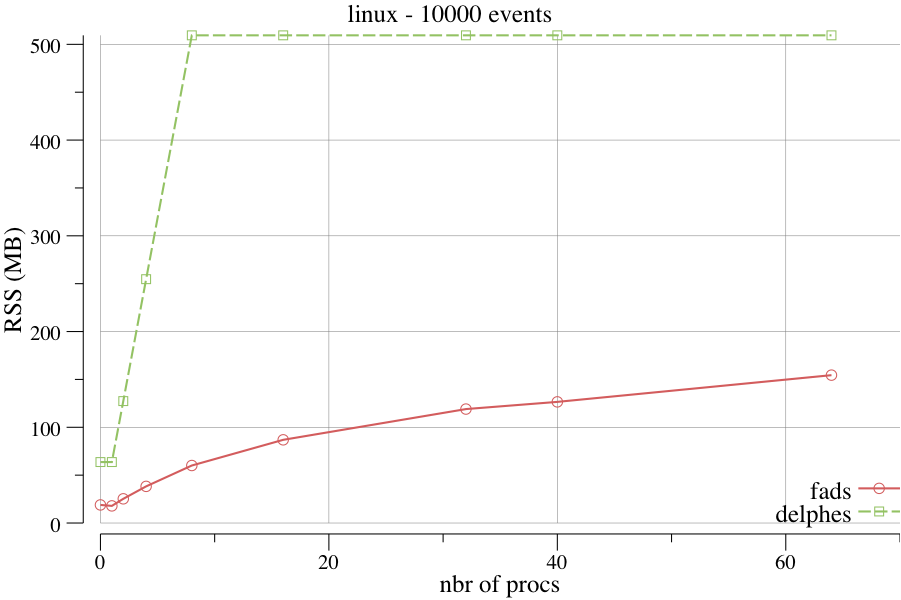
\includegraphics[width=0.95\linewidth]{figs/lhcb3-rss.png}
\end{center}
}

\frame{
  \frametitle{Linux (40 cores) testbench: event throughput}
\begin{center}
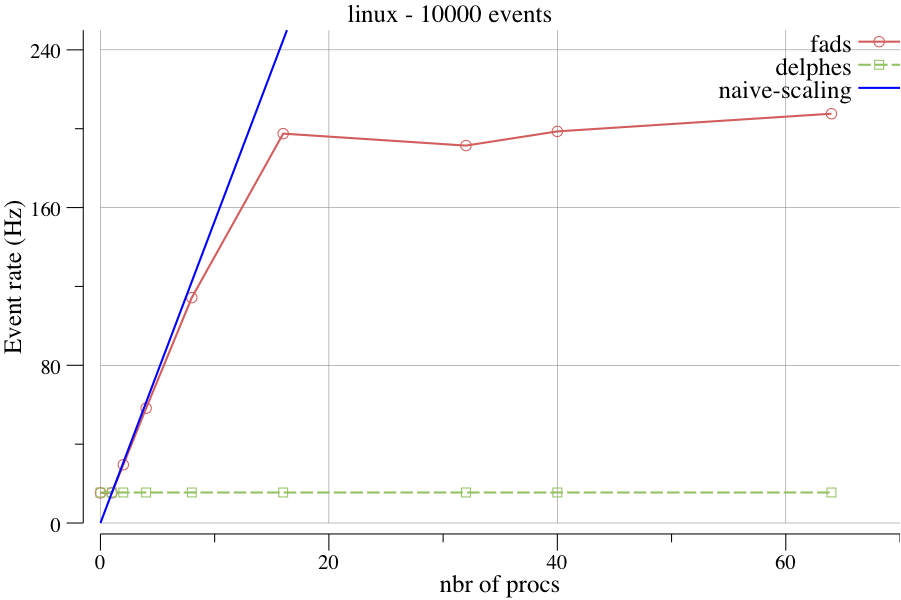
\includegraphics[width=0.95\linewidth]{figs/lhcb3-hz.png}
\end{center}
}

\frame{
  \begin{center}
    \begin{block}{}
      \begin{center}
        \texttt{go-hep}
      \end{center}
    \end{block}
  \end{center}
}

\frame{
  \frametitle{\texttt{go-hep} project}

  A set of pure-\texttt{Go} or bindings to \texttt{HEP} libraries

  \begin{block}{}
    \begin{itemize}
      \item \myblue{\href{https://github.com/go-hep/fads}{\texttt{go-hep/fads}}}: fast detector simulation toolkit
      \item \myblue{\href{https://github.com/go-hep/fastjet}{\texttt{go-hep/fastjet}}}: jet clustering algorithms (\emph{WIP})
      \item \myblue{\href{https://github.com/go-hep/fmom}{\texttt{go-hep/fmom}}}: 4-vectors
      \item \myblue{\href{https://github.com/go-hep/fwk}{\texttt{go-hep/fwk}}}: concurrent framework

      \item \myblue{\href{https://github.com/go-hep/hbook}{\texttt{go-hep/hbook}}}: histograms and n-tuples (\emph{WIP})
      \item \myblue{\href{https://github.com/go-hep/hplot}{\texttt{go-hep/hplot}}}: interactive plotting (\emph{WIP})
      \item \myblue{\href{https://github.com/go-hep/hepmc}{\texttt{go-hep/hepmc}}}: \texttt{HepMC} in \texttt{Go} (EDM + \texttt{I/O})

    \end{itemize}
  \end{block}
}

\frame{
  \frametitle{\texttt{go-hep} + \texttt{astrogo} projects}

  \begin{block}{}
    \begin{itemize}
    \item \myblue{\href{https://github.com/go-hep/hepevt}{\texttt{go-hep/hepevt}}}: \texttt{HEPEVT} bindings
    \item \myblue{\href{https://github.com/go-hep/heppdt}{\texttt{go-hep/heppdt}}}: \texttt{HEP} particle data table
    \item \myblue{\href{https://github.com/go-hep/lhef}{\texttt{go-hep/lhef}}}: Les Houches Event File format
      
    \item \myblue{\href{https://github.com/go-hep/croot}{\texttt{go-hep/croot}}}: bindings to a subset of \texttt{ROOT} \texttt{I/O}
    \item \myblue{\href{https://github.com/go-hep/rio}{\texttt{go-hep/rio}}}: \texttt{go-hep} record oriented \texttt{I/O}
    \item \myblue{\href{https://github.com/go-hep/sio}{\texttt{go-hep/sio}}}: \texttt{LCIO} \texttt{I/O}
    \item \myblue{\href{https://github.com/go-hep/slha}{\texttt{go-hep/slha}}}: \texttt{SUSY} Les Houches Accord \texttt{I/O}
      
\quad\\
    \item \myblue{\href{https://github.com/astrogo/cfitsio}{\texttt{astrogo/cfitsio}}}: bindings to \texttt{FITSIO}
    \item \myblue{\href{https://github.com/astrogo/fitsio}{\texttt{astrogo/fitsio}}}: pure \texttt{Go} \texttt{I/O} for \texttt{FITS} files
    \item \myblue{\href{https://github.com/astrogo/vo}{\texttt{astrogo/vo/votable}}}: \texttt{I/O} for \texttt{VOTable} (\emph{WIP})
      
\quad\\
    \item \myblue{\href{https://github.com/sbinet/go-hdf5}{\texttt{sbinet/hdf5}}}: bindings to \texttt{HDF5}
    \end{itemize}
  \end{block}
}

\frame{
  \frametitle{\texttt{go-hep} \& HSF}
  \begin{block}{}
Most of development workflow already addressed (doc, CI, DVCS)

HSF could provide (from \myblue{\href{https://github.com/go-hep}{\texttt{go-hep}}} POV):

\begin{itemize}
  \item wider audience (users, developers)
  \item  test machines/architectures
  \item  storage area for input data (for tests) and/or (binary) releases
  \item  agreement on \mypurple{cross-language} interoperability (file formats, data layout (\texttt{POD})) in a \mypurple{non pure-\texttt{C++}} environment
\end{itemize}
  \end{block}
}
\end{document}


